\documentclass[a4paper,12pt,titlepage]{article}
%\usepackage[T1]{fontenc}

\usepackage{titlesec}
\usepackage{titling}
\usepackage[portuguese]{babel}
\usepackage[utf8x]{inputenc}
\usepackage{indentfirst}
\usepackage{graphicx}
%\usepackage{times}
\usepackage{ucs}
\usepackage{float}    
\usepackage{fancyvrb}   
\usepackage{verbatim}
\usepackage{listings}
\usepackage{hyperref}
\usepackage{epigraph}
\usepackage{listings}
\usepackage{tabularx}
\usepackage{lipsum}
\usepackage{enumitem}

\hypersetup{
    colorlinks=true,       
    linkcolor=black,          
    citecolor=black,   
    filecolor=black,  
    urlcolor=black  
}

\hyphenation {di-re-cio-na-men-to} 

%\renewcommand*{\familydefault}{\ttdefault}
\lstset{columns=fullflexible,basicstyle=\ttfamily}

\title{\large
Universidade Federal de Minas Gerais \\ \
Instituto de Ciências Exatas \\ \ 
Departamento de Ciência da Computação \\ \
\\[1cm]
Projeto de Final de Curso\\ \
Projeto e Análise de Algoritmos\\ \
\\[1cm]
\textbf{\Large Relatório Final }
\\[1cm]
}

\author{\large Alberto Hideki Ueda \\[0.5cm] 
	Orientador: Berthier Ribeiro Neto 
\\[3cm] }

\date{\textsc{Belo Horizonte\\ \
1º de dezembro de 2014}}

\begin{document}
\maketitle

\pagebreak
\tableofcontents
\pagebreak

\section {O Problema}

\subsection{Contexto}

Coletores de páginas da \textit{Web} constituem o primeiro passo para a implementação de máquinas de busca modernas. De forma geral, um coletor - em inglês, \textit{crawler} - é um sistema que faz requisições a servidores da \textit{Web} de forma planejada e automática, coleta parte ou todo o conteúdo das páginas devolvidas pelas requisições e utiliza este novo conteúdo para realizar novas requisições \cite{b}. Estima-se que hoje mais de 10\% das visitas a \textit{Websites} sejam feitas por coletores \cite{nielsen}.

O primeiro coletor \textit{Web} conhecido foi criado em 1993 por Matthew Gray - então graduando do MIT - e chamava-se WWWW (\textit{World Wide Web Wanderer)}. Comprovando a forte relação com a história dos sistemas de busca na \textit{Web}, no mesmo ano foi lançada também a primeira máquina de busca conhecida, ALIWEB, criada por Martijn Koster \cite{b}. Nesta época, um número razoável de servidores para se obter uma boa cobertura da rede girava em torno de apenas alguns milhares. Desde então, o número de \textit{hosts} tem aumentado em alta velocidade  (chegando a praticamente dobrar a cada ano, de 1993 a 1996 \cite{gray}), tornando as máquinas de busca ainda mais necessárias e, consequentemente, também os coletores de dados.

A figura a seguir mostra o ciclo de funcionamento de um sistema completo, desde a coleta até a busca em si.

\begin{figure}[H]
     \centering
     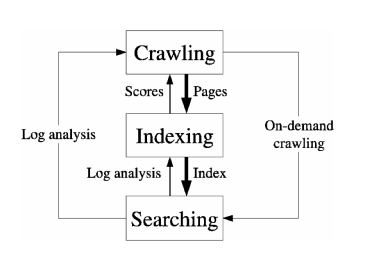
\includegraphics[scale=0.6]{figures/search-engine-cycle.png}
     \caption{Ciclo de uma máquina de busca \cite{carlos}.}
     \label{bsp}
\end{figure}

Deste modo, podemos fazer a seguinte pergunta: como coletar as páginas da \textit{Web} de forma eficiente em termos de tempo e espaço, mantendo um nível mínimo de qualidade do resultado?

\subsection{Dificuldade do Problema}

Hoje, mesmo as principais máquinas de busca cobrem apenas uma parte da \textit{Web} atual. Em 2005, foi demonstrado que o nível de cobertura das principais máquinas de buscas existentes está entre 58\% e 76\% da \textit{Web} \cite{gulli}. Além disso, o custo da utilização da rede também deve ser considerado. Em 2004, tal custo foi estimado em US\$ 1,5 milhão para coletores de larga escala \cite{craswell}. 

Outra característica que torna o problema difícil é a velocidade em que a \textit{Web} se modifica. Devido à facilidade de acesso e à alta disponibilidade de servidores nos dias atuais, a cada minuto novas páginas são criadas, modificadas ou removidas da \textit{Web}. Em todos os casos, a relevância de cada página existente pode aumentar ou diminuir, conforme as novas características da \textit{Web}. A figura abaixo ilustra esta ideia.

\begin{figure}[H]
     \centering
     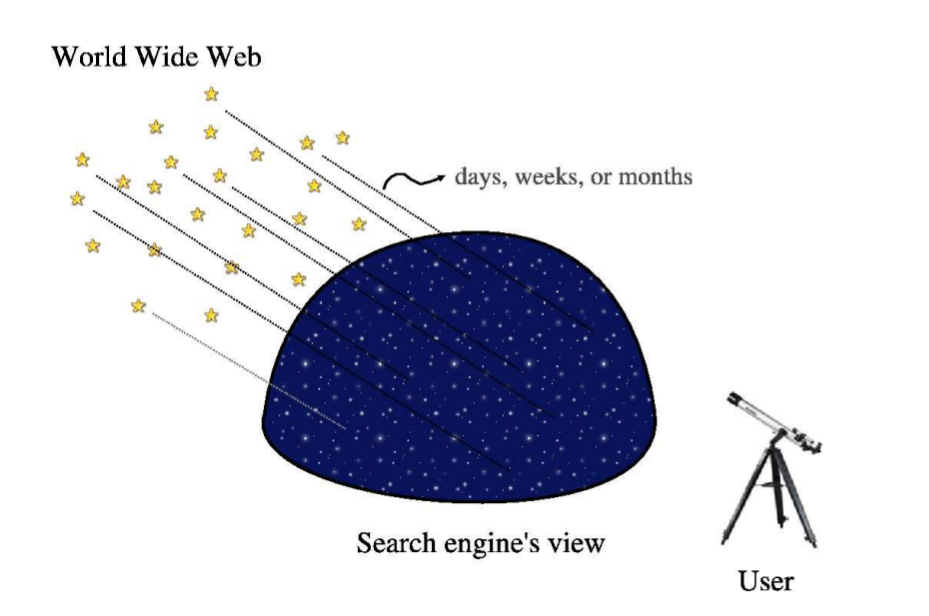
\includegraphics[scale=0.3]{figures/stars.png}
     \caption{coletar documentos da \textit{Web} pode ser visto como analisar um céu estrelado. No momento em que podemos visualizá-lo, o cenário real já se modificou.}
     \label{bsp}
\end{figure}

Portanto, tal problema pode ser considerado de difícil resolução, dado o dinamismo e o tamanho da entrada necessária para uma solução exata.

\subsection{Objetivos do Trabalho}

O objetivo deste trabalho é modificar um algoritmo existente de um \textit{Web Crawler}, construindo uma heurística que visa aumentar a qualidade das páginas coletadas em relação ao algoritmo original, nos casos específicos em que o coletor deve se concentrar em um determinado tópico de interesse.

Mais especificamente, este trabalho consistirá em alterações no escalonamento de longo prazo de um coletor, direcionando as requisições de \textit{downloads} para páginas relevantes a um tópico pré-estabelecido, utilizando na análise de futuros \textit{links} os termos mais frequentes das páginas já coletadas.


\subsection{Abordagem Utilizada}

Para isso, modificaremos a estratégia que o coletor utiliza para determinar quais são os próximos \textit{links} que devem ser processados. No caso do \textit{WIRE}, nosso \textit{baseline}, devemos alterar seu escalonamento de longo-prazo (componente \textit{manager}, descrito na seção 3), substituindo parte do código por um novo algoritmo de escolha das próximas páginas que deverão ser coletadas.

Em seguida, executaremos testes de coleta para os dois algoritmos - original e modificado - e faremos a comparação dos resultados obtidos. Dado um tópico-alvo para a coleta, espera-se que o algoritmo adaptado seja melhor em termos de espaço e memória que o original. Mais tecnicamente, nosso \textit{crawler} deverá encontrar parte das páginas mais relevantes \textit{antes} do coletor do \textit{baseline}. 

%%%%%%%%%%%%%%%%%%%%%%%%%%%%%%%%%%%%%%%%%%%%%%%%%%%%%%%
\section{Modelagem através de um Grafo}
%%%%%%%%%%%%%%%%%%%%%%%%%%%%%%%%%%%%%%%%%%%%%%%%%%%%%%%

Considerando as páginas da \textit{Web} como vértices e os diversos \textit{links} encontrados como arestas, pode-se aplicar diferentes algoritmos para a seleção \textit{on-line} (em tempo de execução) dos \textit{links} que o nosso \textit{crawler} irá visitar em um nova coleta. Possíveis estratégias de escolha (\textit{selection policy}) para o coletor baseiam-se, por exemplo, em: buscas em largura \cite{najork}, indicador \textit{PageRank} \cite{cho} ou até mesmo no uso de algoritmos genéticos \cite{johnson}. 

\begin{figure}[H]
     \centering
     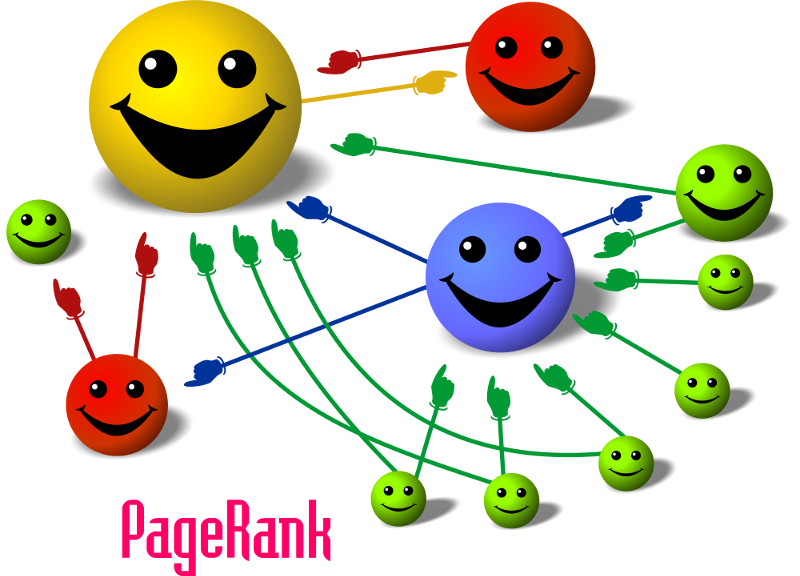
\includegraphics[scale=0.3]{figures/pagerank.png}
     \caption{Um dos indicadores mais conhecidos em recuperação de informação, o \textit{PageRank} mede a relevância de uma página da \textit{Web} considerando, por exemplo, o número de \textit{links} que apontam para esta página e a relevância das origens destes \textit{links}. Na figura, quanto maior o tamanho do círculo (página da \textit{Web}), maior sua relevância.}
     \label{bsp}
\end{figure}

Levando-se em conta que não é possível coletar todas as páginas da \textit{Web}, devido à enorme quantidade de páginas e sua característica mutável, é importante encontrar as páginas mais relevantes o quanto antes. Quanto mais rápido uma página muito relevante for encontrada (de acordo com o indicador considerado), melhor a qualidade dos resultados obtidos em um dado instante de tempo da execução do coletor.

Podemos então pensar no seguinte problema: dado um grafo $G(V,A)$ e um inteiro $k$, em que: 
\begin{itemize}[leftmargin=1.6cm]
    \item os vértices de $G$ são páginas da Web, 
    \item as arestas representam os links entre estas páginas, e
    \item cada vértice possui uma pontuação de relevância não-conhecida a priori,
\end{itemize}
percorrer um caminho que maximiza as pontuações dos vértices visitando no máximo $k$ páginas. \\ 

Desta forma, para a implementação de um \textit{crawler} de alto desempenho, é interessante considerar a estrutura da \textit{Web} atual. Tal estrutura pode ser analisada sob duas perspectivas: \textit{microscópica} e \textit{macroscópica}.

Sob uma perspectiva microscópica, percebe-se que a estrutura dos \textit{links} não se assemelha a um arranjo aleatório. Ao invés disso, é comum identificar \textit{hubs} e redes \textit{scale-free} {\cite{barabasi}}, como ilustrado na figura abaixo.

\begin{figure}[H]
     \centering
     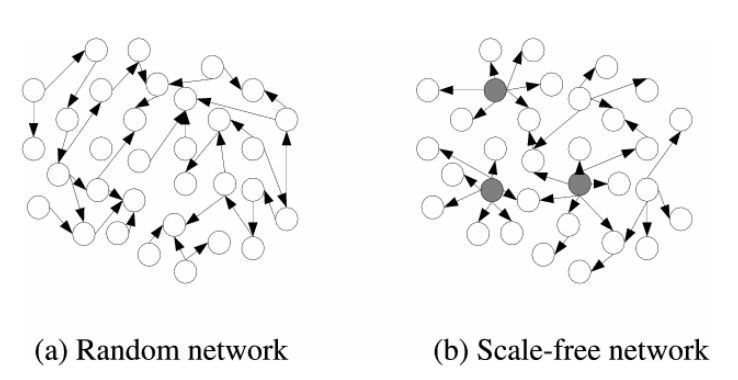
\includegraphics[scale=0.5]{figures/network-types.png}
     \caption{Exemplos de estruturas microscópicas da \textit{Web}. Uma rede gerada aleatoriamente (à esquerda) e uma rede \textit{scale-free} \cite{barabasi}.}
     \label{bsp}
\end{figure}

Já sob a perspectiva macroscópica, podemos identificar uma estrutura \textit{bow-tie} {\cite{broder}}, conforme visto em um dos trabalhos práticos da disciplina. A figura a seguir apresenta uma possível visualização desta estrutura.
 
\begin{figure}[H]
     \centering
     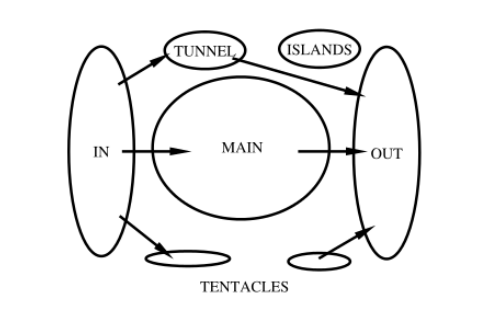
\includegraphics[scale=0.5]{figures/macroscopic-structure-web.png}
     \caption{Estrutura macroscópia da \textit{Web} \cite{broder}.}
     \label{bsp}
\end{figure}

Devido a estas perspectivas, muitos \textit{crawlers} são implementados de modo a beneficiar-se destas informações. Este é o caso do WIRE \cite{carlos}, o \textit{web crawler} que é nosso \textit{baseline} neste trabalho. 

%%%%%%%%%%%%%%%%%%%%%%%%%%%%%%%%%%%%%%%%%%%%%%%%%%%%%%%
\section{Baseline}
%%%%%%%%%%%%%%%%%%%%%%%%%%%%%%%%%%%%%%%%%%%%%%%%%%%%%%%

De forma geral, os coletores podem ser divididos em diversas categorias, conforme mostra a figura a seguir. Em cada categoria é possível identificar quais critérios são os mais importantes em uma coleta. 

\begin{figure}[H]
     \centering
     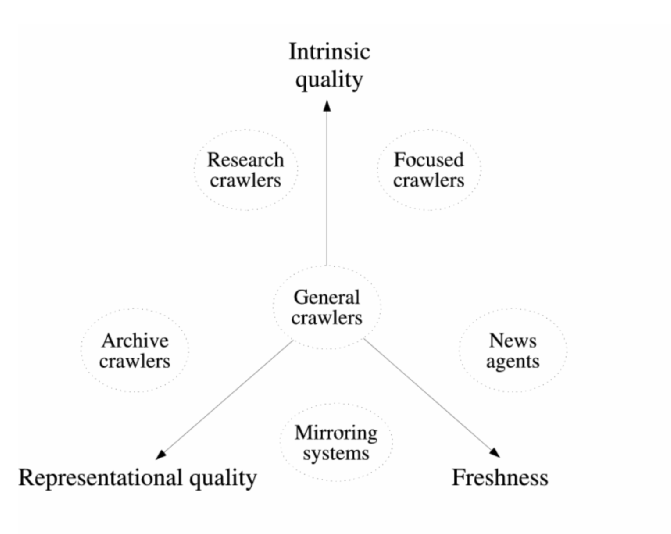
\includegraphics[scale=0.5]{figures/crawlers-types.png}
     \caption{Tipos de coletores \cite{carlos}.}
     \label{bsp}
\end{figure}

Por exemplo, em um coletor que visa reproduzir inteiramente o conteúdo das páginas em determinado instante de tempo, a \textit{qualidade da representação} é o critério mais importante; já o \textit{nível de atualização (freshness)} das páginas não é um critério tão relevante quanto o anterior. 

Nosso baseline, descrito a seguir, é um coletor do tipo genérico. Ou seja, um coletor que tenta equilibrar os três critérios de qualidade, sem focar especificamente em algum destes critérios. Ao invés de apresentar os melhores resultados para um determinado critério, tal coletor tenta garantir um mínimo de qualidade em cada um deles.

\subsection{WIRE}

O \textit{baseline} para este trabalho é o \textit{WIRE} (\textit{Web Information Retrieval Environment}), um \textit{web crawler} desenvolvido por Carlos Castillo em seu doutorado na Universidade do Chile \cite{carlos}. Este coletor foi construído visando-se alto desempenho e boa escalabilidade, respeitando as políticas de restricões a visitas de robôs a servidores \textit{Web}. 

O objetivo principal do \textit{WIRE} é realizar a caracterização da \textit{Web}, a partir dos dados coletados. A figura abaixo é uma representação em alto nível da função do coletor e possíveis integrações com outros objetivos de trabalho, representados em cinza claro.

\begin{figure}[H]
     \centering
     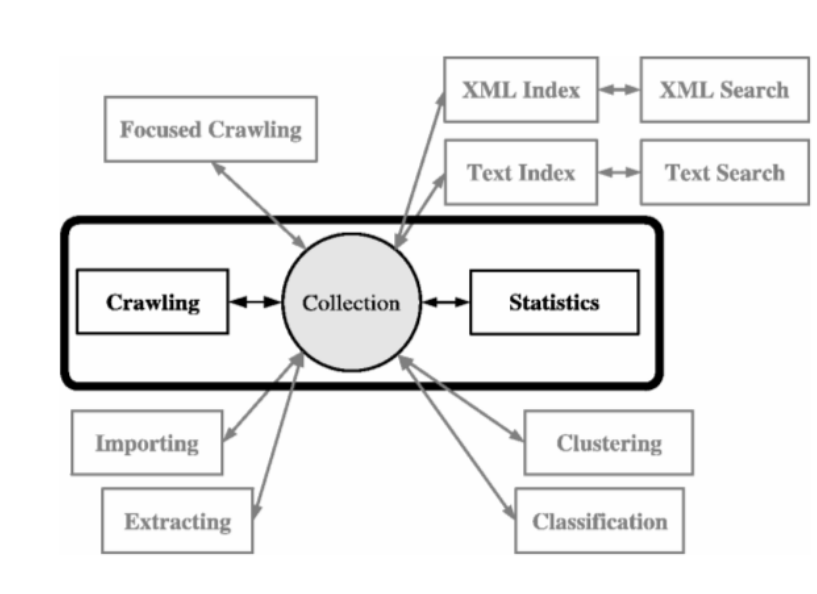
\includegraphics[scale=0.4]{figures/wire-architecture.png}
     \caption{Áreas de atuação do \textit{WIRE} (em preto) e trabalhos futuros (em cinza) \cite{carlos}.}
     \label{bsp}
\end{figure}

\subsection{Algoritmo}

O algoritmo deste \textit{baseline} é representado em alto nível pela figura a seguir.

\begin{figure}[H]
     \centering
     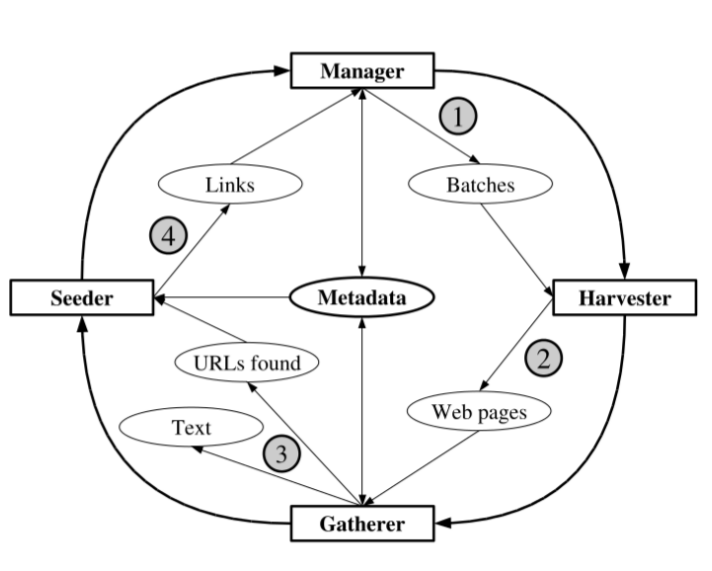
\includegraphics[scale=0.45]{figures/wire-crawling-architecture-2.png}
     \caption{Representação do funcionamento do coletor \textit{WIRE} \cite{carlos}.}
     \label{bsp}
\end{figure}

Cada componente é descrito abaixo: 

\begin{itemize}
\item \textit{Manager}: realiza os cálculos da relevância de cada página coletada e as atualizações no escalonamento de longo-prazo;
\item \textit{Harvester}: responsável pelo escalonamento de curto prazo e pelas coletas de páginas;
\item \textit{Gatherer}: faz o \textit{parse} e a extração de \textit{links};
\item \textit{Seeder}: responsável pela \textit{resolução} de \textit{URLs} e atualizações no grafo de \textit{links};
\end{itemize} 

O algoritmo utiliza listas de adjacências para representar a estrutura de \textit{links} encontrada entre as páginas, podendo ser descrito da seguinte forma:

\begin{enumerate}
\item (\textit{Seeder}) A partir de um arquivo inicial de \textit{URLs}, gera-se a lista das próximas páginas que devem ser coletadas;
\item (\textit{Manager}) Se uma página da lista gerada já foi visitada recentemente, a mesma é ignorada;
\item O valor intrínseco de cada página da lista é calculado, por meio de um indicador. Por exemplo, o \textit{PageRank} \cite{pagerank};
\item Calcula-se o quanto as páginas estão atualizadas;
\item Com o valor intrínseco e o nível de atualização das páginas, calcula-se a qualidade geral de cada página;
\item Extrai-se então da lista as $k$ páginas de maior qualidade, $k$ determinado em um arquivo de configuração;
\item (\textit{Harvester}) Determina-se como as $k$ páginas serão coletadas (observando regras de "bom comportamento" para coletores);
\item Coleta-se todas as páginas de acordo com as regras determinadas no item anterior;
\item (\textit{Gatherer}) As informações coletadas são tratadas, armazenando-se o que é relevante e descartando o restante do material coletado;
\item São enviadas para o \textit{Seeder} as novas \textit{URLs} encontradas nas páginas coletadas e reinicia-se o processo, agora sem a necessidade de arquivos de inicialização.
\end{enumerate}

A seguir, um exemplo de como o \textit{manager} calcula as pontuações de cada \textit{URL} e escolhe as próximas páginas para \textit{download}.

\begin{figure}[H]
     \centering
     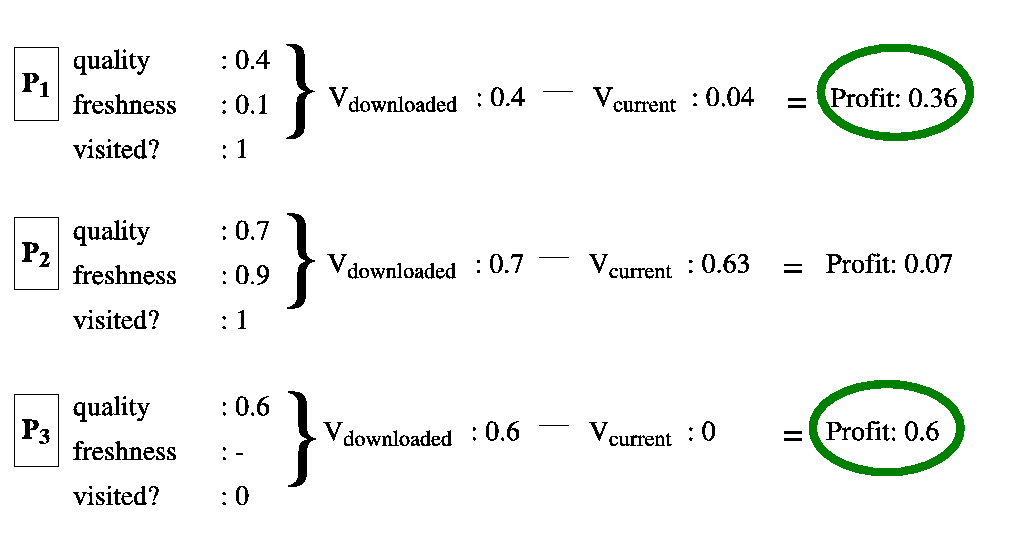
\includegraphics[scale=0.3]{figures/manager.png}
     \caption{Exemplo de escolha do \textit{Manager}. O lucro (\textit{profit}) é a relevância estimada para a página, calculada a partir de seu nível de atualização e indicadores de qualidade como, por exemplo, a relevância das páginas de origem.}
     \label{bsp}
\end{figure}

A condição de parada depende do objetivo do usuário, que pode priorizar cobertura (continuar até que não haja páginas no domínio de interesse, demandando potencialmente um tempo inviável) ou por critério de tempo (encerra-se quando atingir um nível determinado de cobertura). O estudo do \textit{WIRE} mostrou que a partir de uma coleta com 50\% de uma grande coleção de páginas, já é possível atingir 80\% do valor total do \textit{PageRank} dessa coleção \cite{carlos}.

\begin{figure}[H]
     \centering
     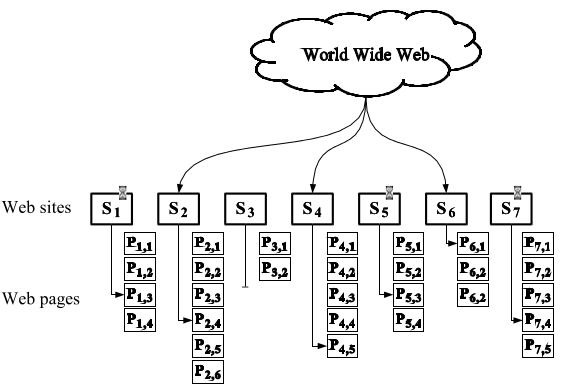
\includegraphics[scale=0.5]{figures/harvester.png}
     \caption{Representação da coleta de \textit{Websites} e suas respectivas páginas, realizada pelo \textit{Wire}.}
     \label{bsp}
\end{figure}


%%%%%%%%%%%%%%%%%%%%%%%%%%%%%%%%%%%%%%%%%%%%%%%%%%%%%%%
\section{Heurística}
%%%%%%%%%%%%%%%%%%%%%%%%%%%%%%%%%%%%%%%%%%%%%%%%%%%%%%%

\subsection{Ideia}

\begin{figure}[H]
     \centering
     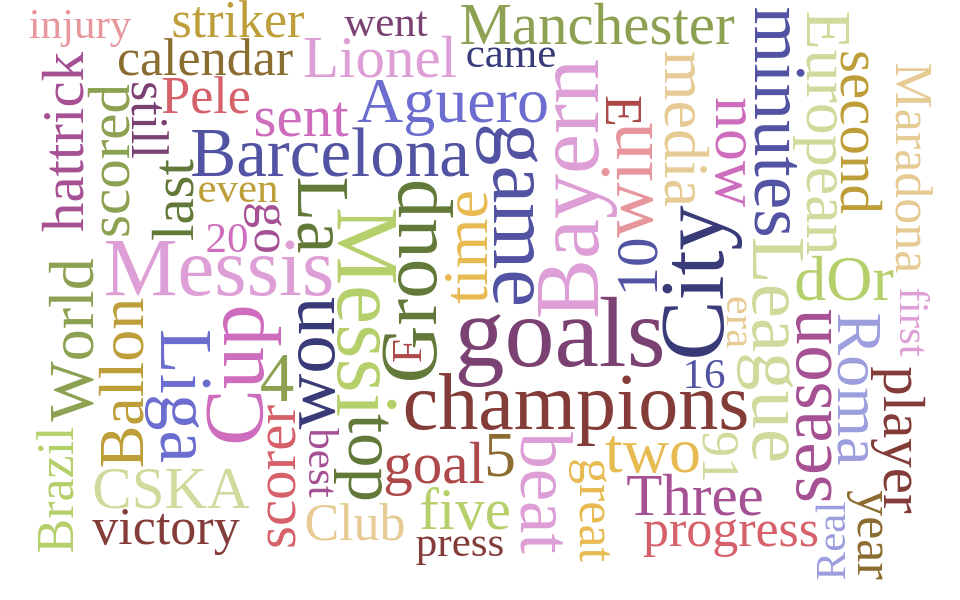
\includegraphics[scale=0.35]{figures/football-cloud.png}
     \caption{http://jasondavies.com/wordcloud.}
     \label{bsp}
\end{figure}

\subsection{Implementação}

Contagem de palavras (Gatherer)
Análise de URL's e Pontuações (Manager)


For the value of an object in the index, V (p), a product function is proposed: \\

$V(p) = IntrinsicQuality(p)^\alpha \ \times \ RepresentationalQuality(p)^\beta \ \times \ Freshness(p)^\gamma$



\section{Análise Teórica de Complexidade}

\begin{figure}[H]
     \centering
     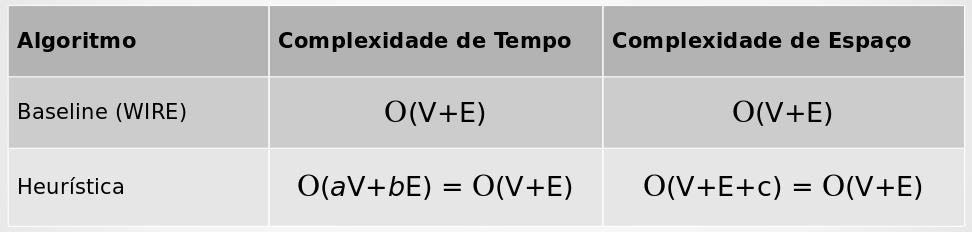
\includegraphics[scale=0.4]{figures/complexity.png}
     \caption{}
     \label{bsp}
\end{figure}

\subsection{Complexidade de Tempo}
\subsection{Complexidade de Espaço}

\section{Análise Experimental dos Algoritmos}
\subsection{Tempo de Execução}
\subsection{Uso de Memória}
\subsection{Qualidade da Resposta}

\begin{figure}[H]
     \centering
     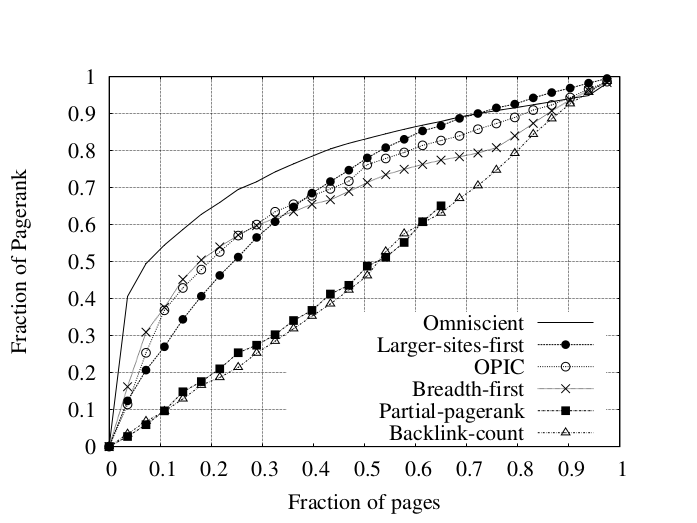
\includegraphics[scale=0.45]{figures/performance.png}
     \caption{Gráfico com os desempenhos de diferentes estratégias para escalonamento de longo prazo  \cite{carlos}.}
     \label{bsp}
\end{figure}

%\subsection{Melhores e Piores Casos}

\section{Trabalhos Futuros}
\section{Conclusão}

% Referências
\bibliographystyle{plain}%amsalpha
\bibliography{bibliografia}
\newpage

\end{document}



\begin{comment}
Na tese de doutorado de Carlos Castillo, diferentes estratégias foram testadas para se medir o desempenho do \textit{WIRE}. Nenhuma leva em conta o caráter temático do coletor, já que o objetivo de seu trabalho era a implementação de um \textit{crawler} de uso geral.
Porém, pode-se ter uma ideia do que esperamos com nosso trabalho visualizando o gráfico a seguir, obtido da tese em que o \textit{WIRE} foi apresentado. Para cada estratégia (linha), quanto antes a mesma atingir o \textit{PageRank} \cite{pagerank} máximo (igual a 1), melhor é a estratégia, como dito na seção de modelagem. Dado um tema específico, nosso \textit{focused crawler} poderá ser representado por uma nova linha no gráfico. É desejado que a mesma esteja acima (encontre as páginas mais relevantes antes) das estratégias do \textit{crawler} original.

\end{comment}



